\section{Semaine 04 (14/10-18/10) }


\e{Notions abordées :}
\begin{itemize}
	\item Mécanique de MPSI (forces centrales).
	\item Dynamique en référentiel non galiléen.
\end{itemize}

\subsection{Exercice 1 : Force en $1/r^4$}

On considère un point matériel de masse $m$ soumis à la force $\vec{F} = \frac{-K}{r^4} \vec{e}_r$, avec $K>0$.

\begin{enumerate}
	\item Montrer que le mouvement est plan et qu'il vérifie la loi des aires.
	\item Définir une énergie potentielle effective et la tracer.
	\item Discuter graphiquement les trajectoires possibles. Justifier. Existe-t-il une trajectoire circulaire ?
\end{enumerate}

\subsection{Exercice 2 : Satellite géostationnaire}

\begin{enumerate}
	\item Définir un satellite géostationnaire et déterminer son orbite. Justifier.
	\item Quel travail faut il fournir pour l'élever en altitude de $\SI{50}{km}$ ? 
	\item L'essence à une énergie spécifique de $\SI{13.1}{kWh/kg}$ et une masse volumique de $\SI{745}{\kilogram\per\cubic\meter}$. En déduire le volume de carburant nécessaire pour effectuer la manœuvre.
\end{enumerate}

\e{Réponses :}
\begin{enumerate}
	\item $\SI{42e3}{km}$
	\item $\SI{5.7e6}{J}$
	\item $\SI{0.13}{kg}$ et $\SI{0.16}{\liter}$.
\end{enumerate}

\subsection{Exercice 3 : Chute d'un satellite dans l'atmosphère}

\begin{enumerate}
	\item Un satellite est en orbite circulaire autour de la Terre. Montrer qu'il existe une relation simple entre $E_c$ et $E_p$. Exprimer l'énergie mécanique en fonction de $r$.
	\item Comment évolue la vitesse d'un satellite freiné par l'atmosphère ?
	\item Son altitude est $h=\SI{180}{km}$ et la force de frottement a pour norme $\beta m v^2 / h$.
	\begin{enumerate}
		\item Préciser l'unité de $\beta$.
		\item Déterminer la variation d'altitude $\Delta h$ après une révolution. On proposera les hypothèses appropriées.
	\end{enumerate}
\end{enumerate}

\e{Réponse :} $\Delta h = \SI{-28.3}{m}$.

\subsection{Exercice 4 : Pendule pesant dans une voiture accélérée}

Une tige homogène de longueur $l$ et de masse totale $m$ est accrochée en un point $A$ du plafond d'une voiture. La voiture est en translation rectiligne d'accélération $a$ par rapport au référentiel terrestre supposé galiléen. 

Le moment d'inertie de la tige par rapport au point $A$ est $J = \frac{1}{3}m l ^2$. On admet que le point d'application de la force d'inertie d'entraînement est le centre d'inertie de la tige.

\begin{enumerate}
	\item Déterminer l'angle d'équilibre du pendule dans le référentiel de la voiture.
	\item Déterminer la période $T$ des petites oscillations du pendule autour de la position d'équilibre.
\end{enumerate}

\subsection{Exercice 5 : Limite de Roche}

\begin{minipage}[c]{\linewidth/2}
	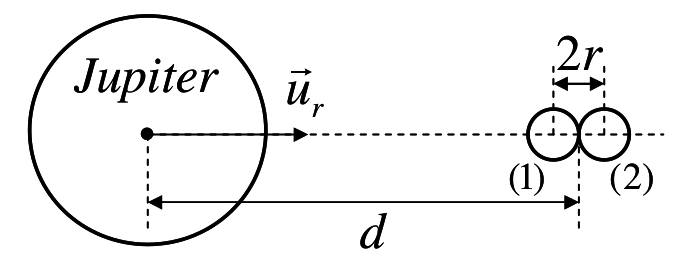
\includegraphics[width=\linewidth]{Images/mp_s04_ex02.png}
\end{minipage}%
\begin{minipage}[c]{\linewidth/2}
	On cherche à déterminer la distance en dessous de laquelle une comète s'approchant de Jupiter se sépare en plusieurs morceaux sous l'effet des forces de marée dues à Jupiter.
	
	On modélise la comète par deux sphères identiques de masses $m$ et de rayon $r$, alignées comme sur le dessin. On suppose que la comète est en orbite circulaire de rayon $d$ autour de Jupiter.
\end{minipage} 

\begin{enumerate}
	\item Montrer que le mouvement du centre d'inertie de la comète est uniforme. Quelle est la nature du mouvement du référentiel de la comète par rapport au référentiel de Jupiter ?
	\item Soit $\vec{R}$ la réaction de la sphère $(1)$ sur la sphère $(2)$. Dans le référentiel de la comète, appliquer le PFD à une des deux sphères.
	\item À quelle condition le contact entre les sphères est-il rompu ? Déterminer, sachant que $r \ll d$, la distance limite $d_{lim}$ en dessous de laquelle il ne peut exister de comètes.
\end{enumerate}

\e{Données :} $M_J = \SI{1.9e27}{kg}$, $R_J = \SI{7.1e4}{km}$ et masse volumique de la comète $\rho_c = \SI{1.0e3}{\kilogram\per\cubic\metre}$.

\e{Réponse :} $d_{lim} = \SI{1.8e5}{km}$.

\subsection{Exercice 6 : Usure d'une ligne de TGV}

Un train grande vitesse se dirige vers le sud, depuis Paris (latitude $48.8$°). On considère son mouvement dans le référentiel terrestre non galiléen. Montrer qu'apparaît une réaction horizontale de la voie sur le train. La comparer à la réaction verticale. 


\subsection{Exercice 7 : Impesanteur}

Existe-t-il un endroit où $\vec{g} = \vec{0}$ ? Commenter la valeur numérique obtenue.

\e{Réponse :} $\SI{42e3}{km}$